\documentclass[9pt,twocolumn,twoside,]{pnas-new}

% Use the lineno option to display guide line numbers if required.
% Note that the use of elements such as single-column equations
% may affect the guide line number alignment.


\usepackage[T1]{fontenc}
\usepackage[utf8]{inputenc}

% tightlist command for lists without linebreak
\providecommand{\tightlist}{%
  \setlength{\itemsep}{0pt}\setlength{\parskip}{0pt}}


% Pandoc citation processing
%From Pandoc 3.1.8
% definitions for citeproc citations
\NewDocumentCommand\citeproctext{}{}
\NewDocumentCommand\citeproc{mm}{%
  \begingroup\def\citeproctext{#2}\cite{#1}\endgroup}
\makeatletter
 % allow citations to break across lines
 \let\@cite@ofmt\@firstofone
 % avoid brackets around text for \cite:
 \def\@biblabel#1{}
 \def\@cite#1#2{{#1\if@tempswa , #2\fi}}
\makeatother
\newlength{\cslhangindent}
\setlength{\cslhangindent}{1.5em}
\newlength{\csllabelwidth}
\setlength{\csllabelwidth}{3em}
\newenvironment{CSLReferences}[2] % #1 hanging-indent, #2 entry-spacing
 {\begin{list}{}{%
  \setlength{\itemindent}{0pt}
  \setlength{\leftmargin}{0pt}
  \setlength{\parsep}{0pt}
  % turn on hanging indent if param 1 is 1
  \ifodd #1
   \setlength{\leftmargin}{\cslhangindent}
   \setlength{\itemindent}{-1\cslhangindent}
  \fi
  % set entry spacing
  \setlength{\itemsep}{#2\baselineskip}}}
 {\end{list}}
\usepackage{calc}
\newcommand{\CSLBlock}[1]{#1\hfill\break}
\newcommand{\CSLLeftMargin}[1]{\parbox[t]{\csllabelwidth}{#1}}
\newcommand{\CSLRightInline}[1]{\parbox[t]{\linewidth - \csllabelwidth}{#1}\break}
\newcommand{\CSLIndent}[1]{\hspace{\cslhangindent}#1}


\templatetype{pnasresearcharticle}  % Choose template

\title{Dynamique des communautés}

\author[a]{Kyara Boisvert}
\author[a]{Zoé Chol}
\author[a]{William Simard}

  \affil[a]{Université de Sherbrooke, Département d'écologie, 2500
Boulevard de l'Université, Sherbrooke, Québec, J1N 3C6}


% Please give the surname of the lead author for the running footer
\leadauthor{}

% Please add here a significance statement to explain the relevance of your work
\significancestatement{}


\authorcontributions{}



\correspondingauthor{\textsuperscript{} }

% Keywords are not mandatory, but authors are strongly encouraged to provide them. If provided, please include two to five keywords, separated by the pipe symbol, e.g:
 \keywords{  abondance |  taxonomie |  communautés |  séries
temporelles  } 

\begin{abstract}
La Terre sert d'habitat pour plusieurs espèces et chacune d'entre eux
ont une importance. Les écosystèmes retrouvés sur notre planète
permettent d'assurer la survie des êtres humains. Cependant, plusieurs
personnes ont des désirs plus grand que la survie, ce qui cause la
destruction des écosystèmes, causant ainsi des déclins dans les
différentes populations ou même l'extinction de certaines espèces. De
cette façon, des études sur la biodiversité son possible afin d'observer
l'état de celle-ci pour ensuite sensibiliser, conserver et préserver les
écosystèmes. Aussi, des analyses statistiques permettent d'obtenir de
l'information importantes afin de confirmer ou d'infirmer des prémisses.
\end{abstract}

\dates{This manuscript was compiled on \today}
\doi{\url{www.pnas.org/cgi/doi/10.1073/pnas.XXXXXXXXXX}}

\begin{document}

% Optional adjustment to line up main text (after abstract) of first page with line numbers, when using both lineno and twocolumn options.
% You should only change this length when you've finalised the article contents.
\verticaladjustment{-2pt}



\maketitle
\thispagestyle{firststyle}
\ifthenelse{\boolean{shortarticle}}{\ifthenelse{\boolean{singlecolumn}}{\abscontentformatted}{\abscontent}}{}

% If your first paragraph (i.e. with the \dropcap) contains a list environment (quote, quotation, theorem, definition, enumerate, itemize...), the line after the list may have some extra indentation. If this is the case, add \parshape=0 to the end of the list environment.

\acknow{}

À travers le temps, nos écosystèmes se sont formés grâce à une grande
diversité d'espèces animales et végétales. Cette richesse spécifique,
retrouvé sur Terre, est intrinsèquement et de manière pragmatique
essentiel à la survie des êtres humains (1). Malgré la reconnaissance de
ces faits et des efforts de conservations constants au maintient de la
biodiversité, elle continue de décliner à un rythme alarmant (1, 2).
Plusieurs populations largement répandues ainsi que des espèces menacées
sont en déclins (3). Combiné avec l'exploitation humaine des écosystèmes
terrestres et des écosystèmes marins, ses facteurs en résultent en un
biotope Terrestre qui est utilisé au delà de sa durabilité (1). À la
suite d'analyses statistiques et d'observations d'une banque de données
d'une série temporelle comportant des échantillonnages entre les années
1950 et 2020, incluant une variété de taxon végétal et animal, nous en
sommes arrivé à trois questions de recherche. La première est :
Observe-t-on un déclin de la biodiversité à travers les années? La
deuxième question est : Quel taxon a-t-on le plus et le moins observé à
travers les années? Puis la dernière est : Quel taxon a le plus décliné
depuis les années 1970? Pour répondre à ces questions, nous avons
effectuées d'autres analyses statistiques évaluant l'abondance des
différentes espèces retrouvées à travers les années. Avec la répartition
de l'abondance des espèces, elle nous permet d'obtenir des preuves sur
le niveau de rareté (ou non) d'une espèce particulière selon d'autres
espèces (4).

\section{Méthodes}\label{muxe9thodes}

Afin de réaliser les analyses statistiques, la banque de données, nommée
séries temporelles, a été fourni par Biodiversité Québec. Ces données
ont été récoltées sur plusieurs décennies, de 1950 à 2020. Cette banque
nous a permis de réaliser plusieurs analyses statistiques. Pour débuter,
nous avons importé les données taxonomiques dans le logiciel R. Par la
suite, nous avons procédé par un nettoyage de l'information de manière à
avoir une base précise. Ensuite, une analyse statistique a été fait dans
le but de créer des data frame contenant les éléments, tel que les noms
scientifiques, les années, les coordonnées, les sources qui procuraient
l'information, etc. Ces data frame ont permis de créer de nouvelles
bases de données utilisées dans logiciel SQL de R studio. Puis ces
nouveaux data frame ont été utilisés pour créer les figures trois
figures suivantes. La Figure \ref{fig:esp.annee} a été conçue à l'aide
de la fonction ``plot''. Le type de lignes, l'épaisseur de la ligne
ainsi que la couleur de celle-ci ont été défini selon les
caractéristiques désirées. Ce graphique représente la richesse
spécifique par année selon le nombre d'espèces observées. La Figure
\ref{fig:obs.classe}, est un graphique à barres (fonction ``bar plot'')
qui représente les différentes classes taxonomiques ainsi que le nombre
d'observation sur une échelle logarithmique. Des caractéristiques
spécifiques tel que la couleur des bandes et leurs bordures ont été
attribués. La Figure \ref{fig:declin} est aussi un graphique à barres
représentant les variations, en pourcentage, des espèces observées selon
les différentes classes à partir des années 1970. Les bandes rouges
représentent les diminutions en abondances des espèces et les bandes
vertes sont les augmentations depuis 1970 selon chaque classes
taxonomiques observées.

\section{Résultats}\label{ruxe9sultats}

Les analyses ont démontré qu'il y a eu une augmentation dans la richesse
des espèces entre les années 1950 et \textasciitilde{} 1993 (Figure
\ref{fig:esp.annee}). De plus, nous observons une forte augmentation du
nombre d'espèces observées lors des années 1970. Cependant, nous pouvons
aussi voir un déclin dans l'abondance des espèces à partir de l'année
1995. À la suite de cette année, 1995, il y a quelques hausses d'espèces
observées, mais de façon générale on remarque un déclin qui s'aggrave
d'années en années.

\begin{figure}
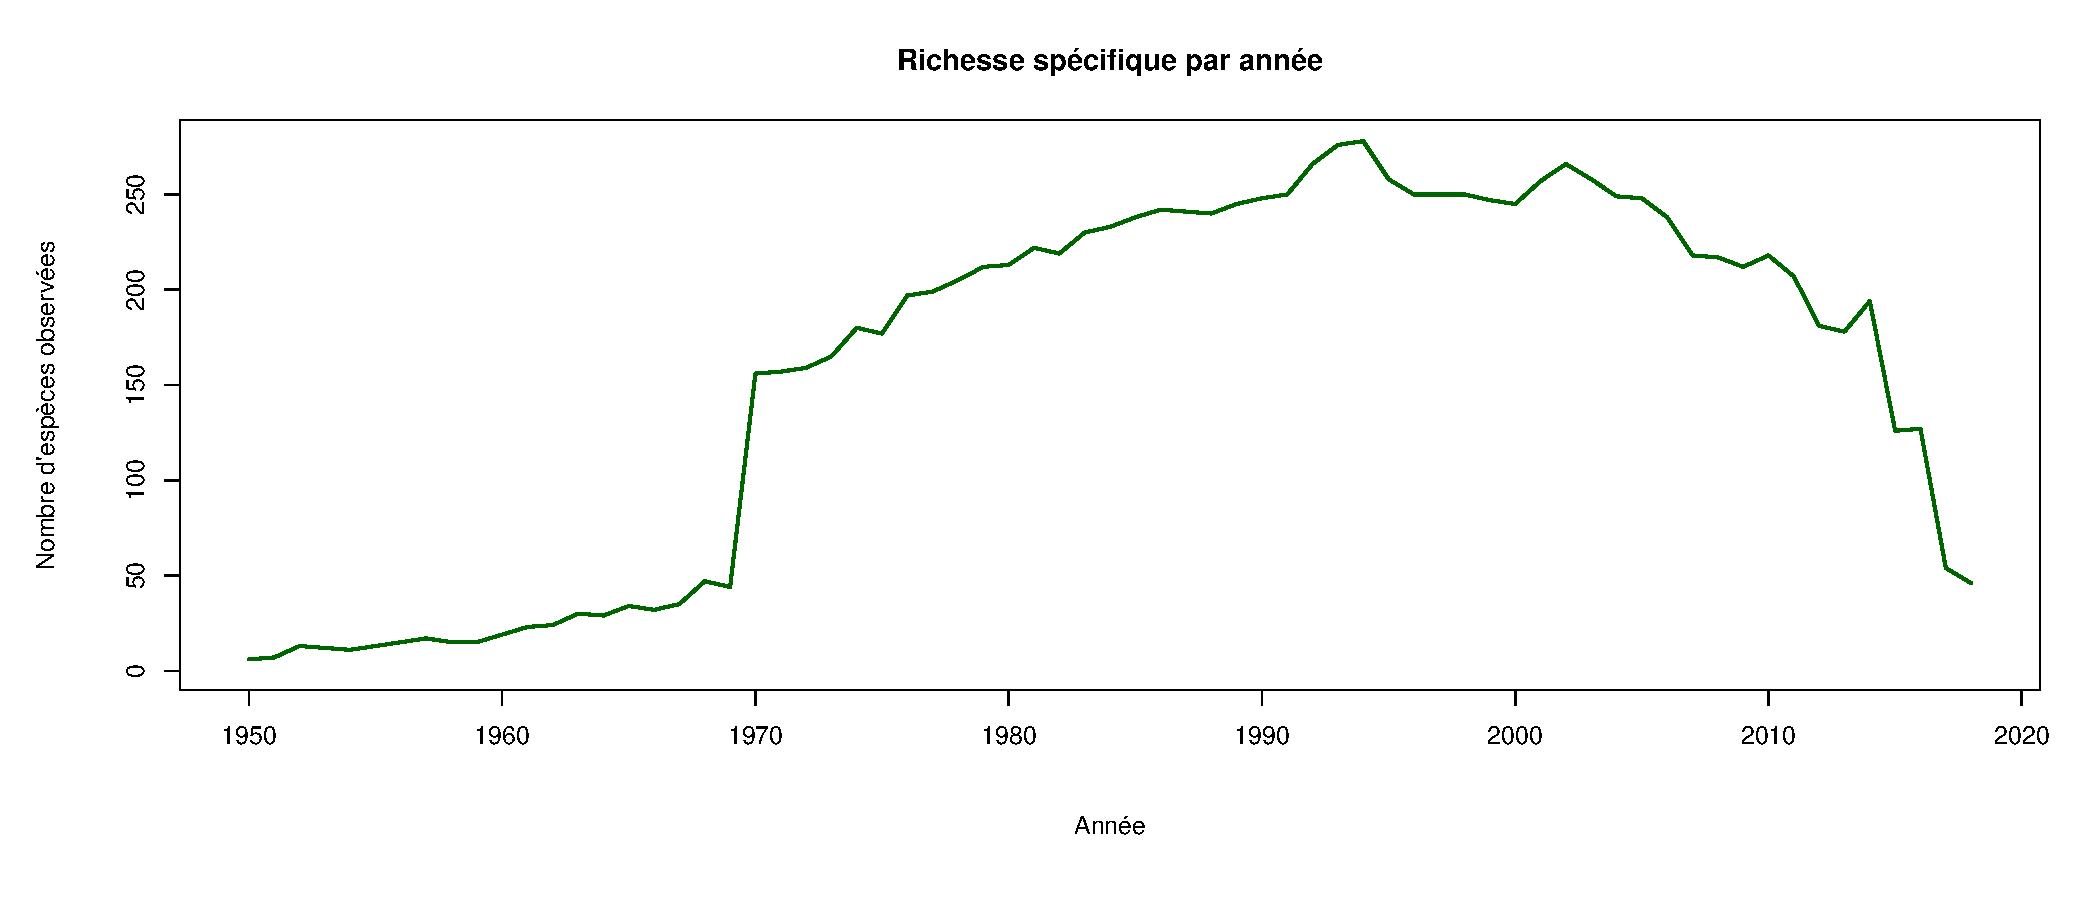
\includegraphics[width=1\linewidth]{Figures/figure_1_esp_par_annee} \caption{\label{fig:esp.annee} Richesse spécifique par année}\label{fig:fig.esp.annee}
\end{figure}

On observe aussi à la Figure \ref{fig:obs.classe} les observations par
classe taxonomique sur une échelle logarithmique. La classe qui a le
plus grand nombre total d'observations est les Teleosteis. En revanche,
celle qui en a le moins est les Petromyzontis.

\begin{figure}
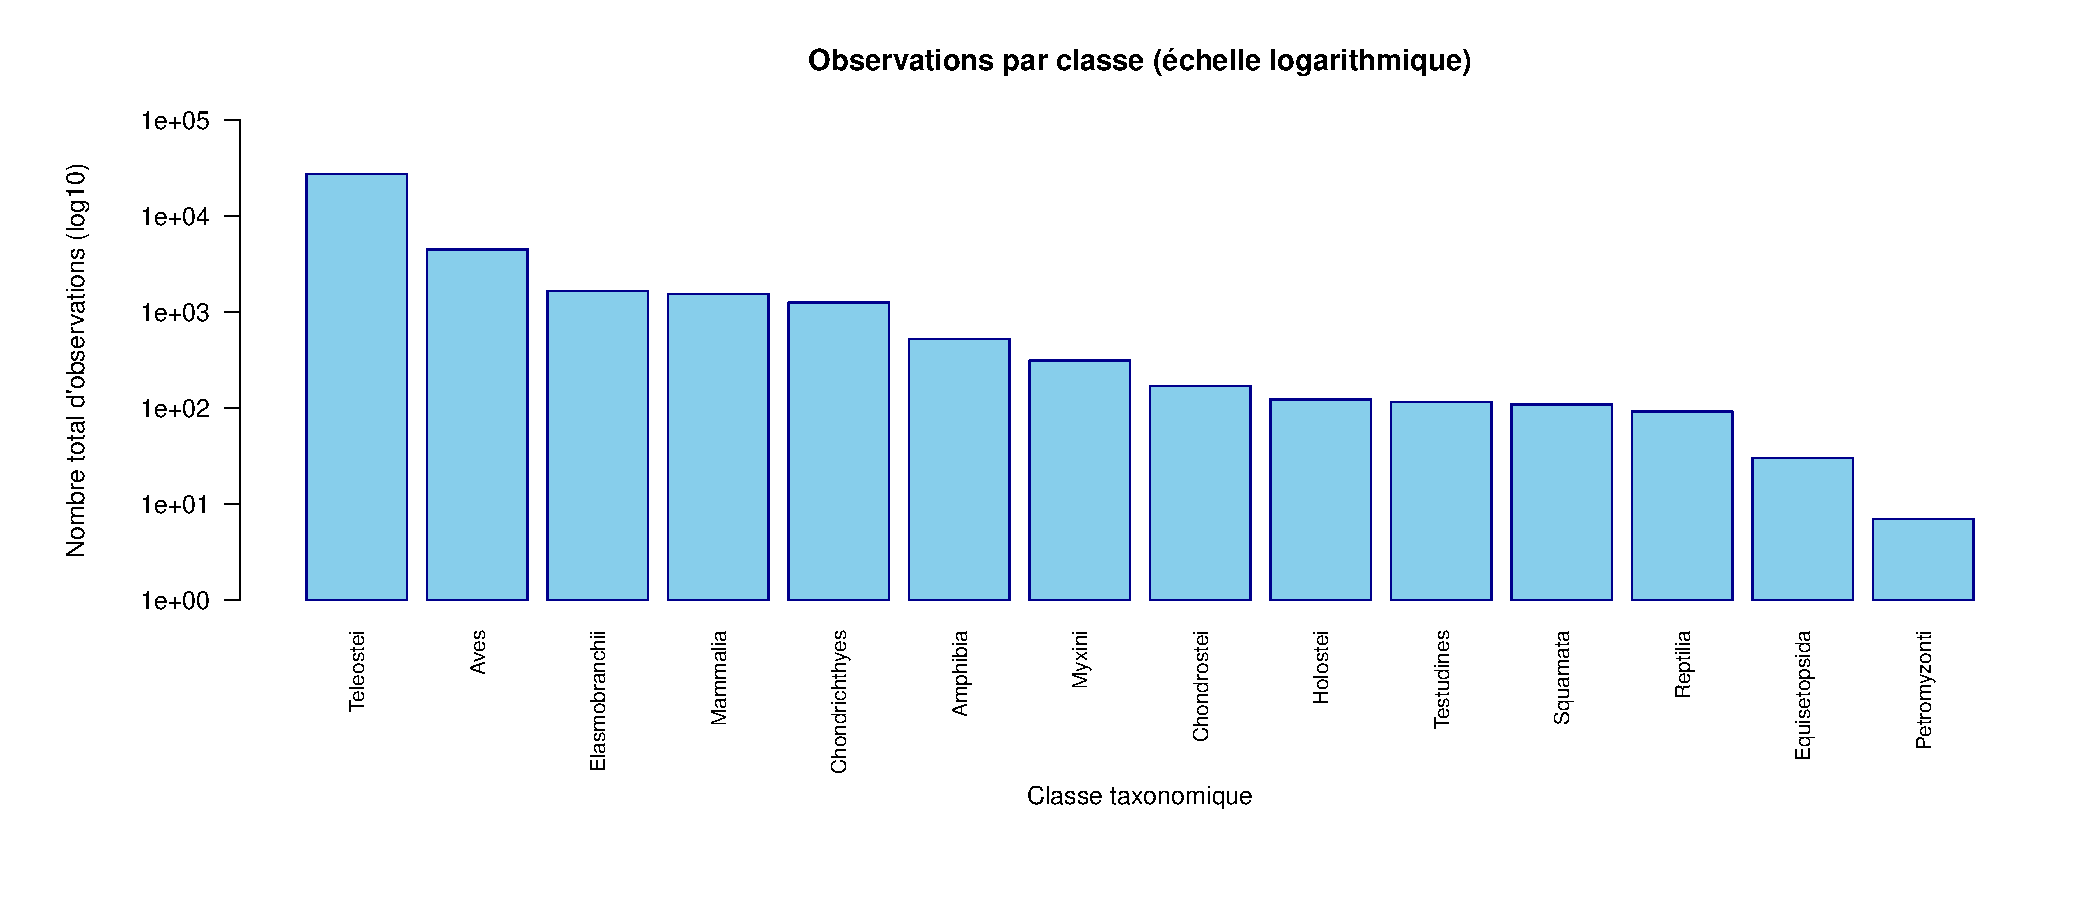
\includegraphics[width=1\linewidth]{Figures/figure_2_obs_par_classe} \caption{\label{fig:obs.classe} Observations par classe (échelle logarithmique)}\label{fig:fig.obs.classe}
\end{figure}

On observe finalement les variations en pourcentage des différentes
classes taxonomiques depuis les années 1970 (Figure \ref{fig:declin}).
Les bandes vertes sont des valeurs positives démontrant une augmentation
du nombre d'observations d'espèces de cette classe et les bandes rouges
sont des diminutions dans le nombre d'observations, donc des valeurs
négatives. Pour cette figure, la classe des Amphibia est celle qui a la
plus grande variation (500\%). Les classes Chondrostei et Equisetopsida
ont une valeur respective de 100\%. Dans les valeurs négatives, on
constate que la classe Aves est celle qui a la plus grande diminution
avec une valeur de - 99\%. Nous pouvons aussi observer une valeur de 0
pour la classe des Petromyzontis.

\begin{figure}
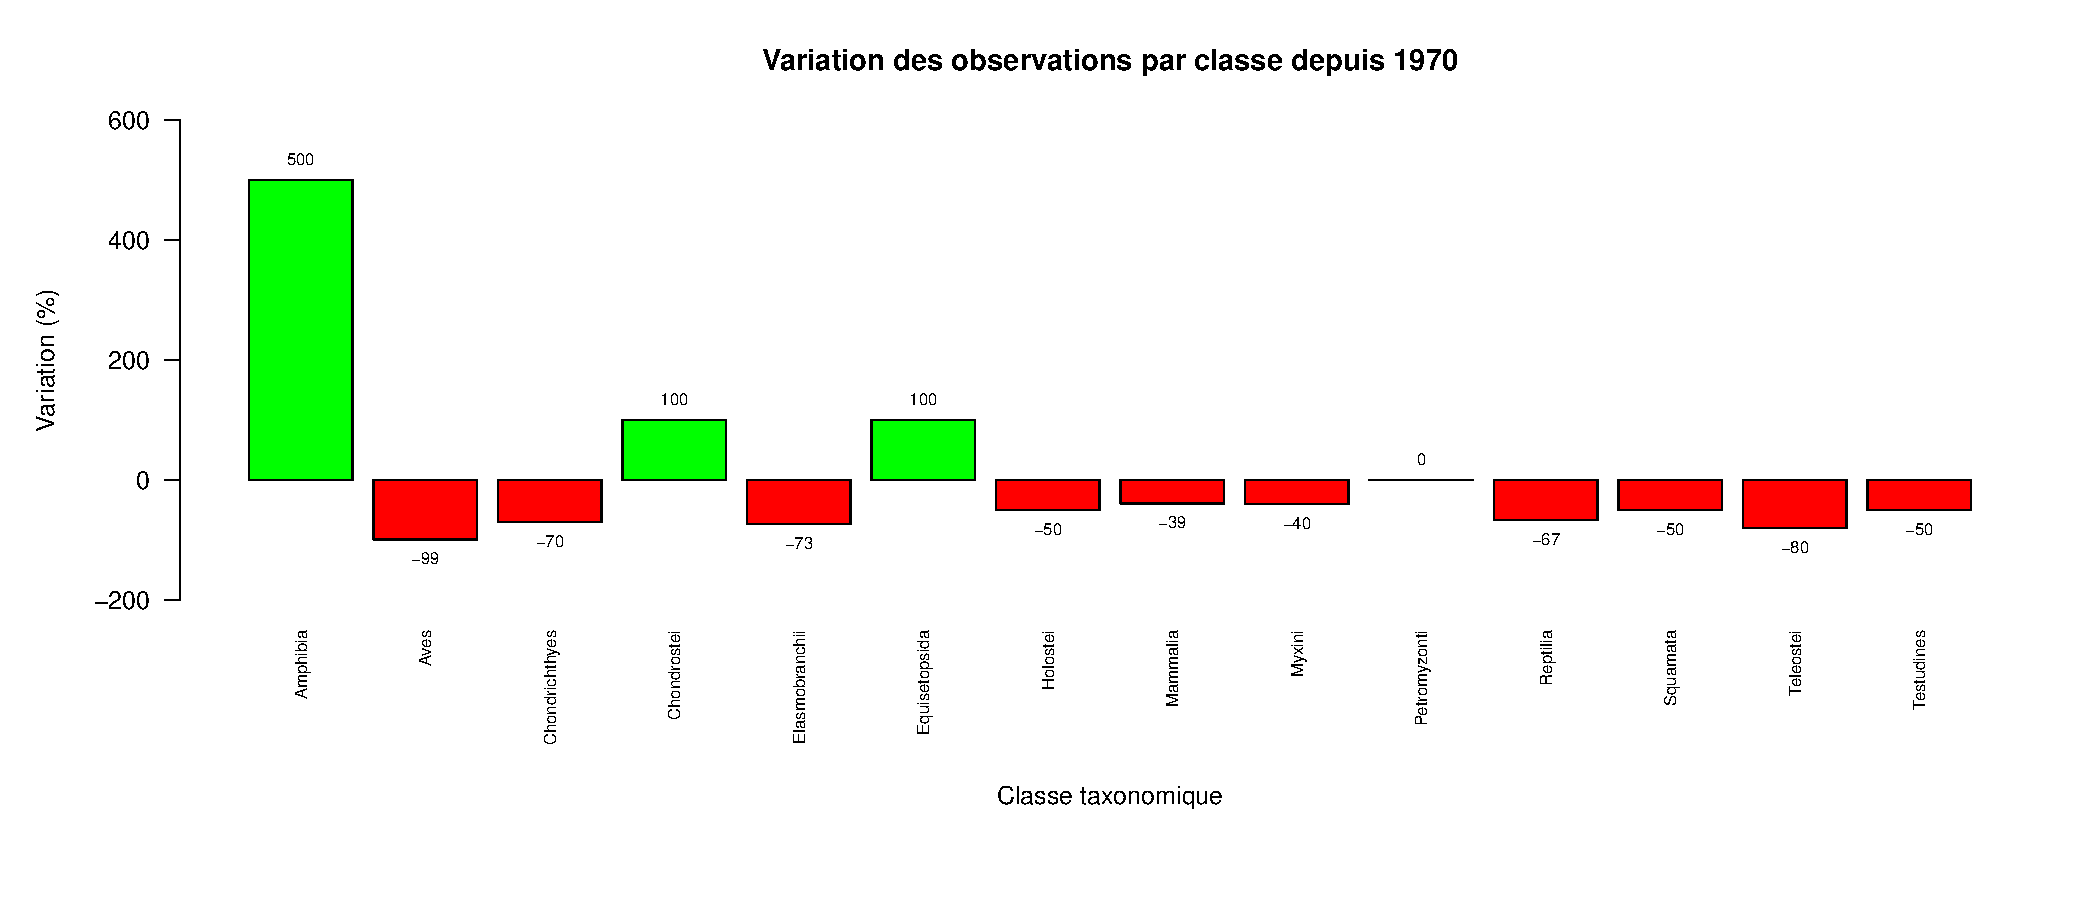
\includegraphics[width=1\linewidth]{Figures/figure_3_declin_classe} \caption{\label{fig:declin} Variation des observations par classe depuis 1970}\label{fig:fig.declin}
\end{figure}

\section{Discussion}\label{discussion}

En ce qui concerne la première question de recherche, observe-t-on un
déclin de la biodiversité à travers les années, la Figure
\ref{fig:esp.annee} est la clé pour répondre. Nous remarquons qu'entre
les années 1950 à 1970 le nombre d'espèces observées est plus faible que
les années suivantes. Cette faible augmentation, dans les observations,
peut être reliées à un manque d'échantillonnage de la part des
chercheurs ou simplement qu'aux endroits étudiés l'abondance des espèces
étaient moins prononcées. De plus, à l'année 1970 il y a une hausse dans
le nombre d'observations de manière drastique. Cette hausse ce fait de
façon constante jusqu'aux années 1990 et plus précisément 1993/1994. À
partir de ces années, un déclin dans la richesse spécifique est visible.
Ce déclin peut être relié à l'endroit où les données ont été récoltées.
Par exemple, l'impact sur la biodiversité diffère selon les biomes
étudiés. Les biomes les plus sous représentés sont les forêts boréales,
les toundras, les prairies inondées, les savanes ainsi que les mangroves
(2). Donc, les espèces retrouvées dans ces milieux sont sujettes à un
biais de l'emplacement de leur habitat. De plus, depuis les années 1980
des préoccupations sont levées à propos de la vitesse à laquelle les
espèces sont perdues de leurs écosystèmes (5). Qui plus est, sur le
graphique de la Figure \ref{fig:esp.annee}, nous remarquons une
diminution constante dans le nombre d'observation à partir des années
2000. Donc, un déclin dans la biodiversité à travers le temps est
observé et ce déclin est causé par l'activité humaine (4).

Pour répondre à la deuxième question de recherche qui consiste à
déterminer quel taxon à été le plus et le moins observé à travers les
années, la Figure \ref{fig:obs.classe} est à la base de la réponse. La
classe avec le plus grand nombre d'observations est celle des Teleosteis
et celle ayant le moins d'observations est les Petromyzontis. Cependant,
le nombre d'observations ne reflète pas nécessairement l'abondance.
Comme les unités de mesure d'abondance n'étaient pas les mêmes d'une
classe à l'autre, il a fallu utiliser le nombre d'observations seulement
pour pouvoir comparer les taxons entre eux.

Dans le but de répondre à la dernière question de recherche, étant quel
taxon à le plus décliné depuis les années 1970, nous allons utiliser la
Figure \ref{fig:declin}. Dans cette figure, nous pouvons observer les
variations du nombre d'observations selon la classe entre l'année 1970
et la dernière année pour laquelle nous avions une observation pour
chaque classe respectivement. La classe démontrant le plus grand déclin
est celle des Aves, les oiseaux. Une diminution de 99\% est observée.
Toutefois, les données pour créer ce graphique incluent seulement les
observations depuis les années 1970, puisqu'entre 1950 et 1970 il y
avait très peu d'échantillons récoltés. Alors, en considérant les
données depuis 1970 un biais dans l'analyse est créé. Comme démontré
dans la littérature, les activités anthropiques ne font qu'accélérer le
déclin dans l'abondance des espèces (4). Ce déclin est de plus en plus
observé depuis les années 2010 où la biodiversité, à l'échelle
terrestre, diminue grandement et rapidement (5).

\section{Conclusion}\label{conclusion}

Pour conclure, à travers le temps nous pouvons observé une diminution
dans la richesse spécifique des différentes espèces retrouvées dans les
écosystèmes terrestre. Selon leur environnement, certaines espèces sont
plus susceptibles que d'autres à un déclin dans leur population. Malgré,
la reconnaissance des effets anthropiques sur les écosystèmes et leurs
espèces, l'Homme doit continuer à s'améliorer afin d'assurer la
conservation et la préservation des biomes.

\section*{Bibliographie}\label{bibliographie}
\addcontentsline{toc}{section}{Bibliographie}

\pnasbreak

\phantomsection\label{refs}
\begin{CSLReferences}{0}{1}
\bibitem[\citeproctext]{ref-kissling_building_2018}
\CSLLeftMargin{1. }%
\CSLRightInline{Kissling WD, et al. (2018)
\href{https://doi.org/10.1111/brv.12359}{Building essential biodiversity
variables of species distribution and abundance at a global scale}.
\emph{Biological Reviews} 93(1):600--625.}

\bibitem[\citeproctext]{ref-newbold_has_2016}
\CSLLeftMargin{2. }%
\CSLRightInline{Newbold T, et al. (2016)
\href{https://doi.org/10.1126/science.aaf2201}{Has land use pushed
terrestrial biodiversity beyond the planetary boundary? {A} global
assessment}. \emph{Science} 353(6296):288--291.}

\bibitem[\citeproctext]{ref-tittensor_mid-term_2014}
\CSLLeftMargin{3. }%
\CSLRightInline{Tittensor DP, et al. (2014)
\href{https://doi.org/10.1126/science.1257484}{A mid-term analysis of
progress toward international biodiversity targets}. \emph{Science}
346(6206):241--244.}

\bibitem[\citeproctext]{ref-matthews_review_2015}
\CSLLeftMargin{4. }%
\CSLRightInline{Matthews TJ, Whittaker RJ (2015)
\href{https://doi.org/10.1111/1365-2664.12380}{{REVIEW}: {On} the
species abundance distribution in applied ecology and biodiversity
management}. \emph{Journal of Applied Ecology} 52(2):443--454.}

\bibitem[\citeproctext]{ref-cardinale_biodiversity_2012}
\CSLLeftMargin{5. }%
\CSLRightInline{Cardinale BJ, et al. (2012)
\href{https://doi.org/10.1038/nature11148}{Biodiversity loss and its
impact on humanity}. \emph{Nature} 486(7401):59--67.}

\end{CSLReferences}



% Bibliography
% \bibliography{pnas-sample}

\end{document}
